\section{Auswertung}
\label{sec:Auswertung}
Aufgrund der Menge an Daten sind die Datensätze nicht im Protokoll mit angegeben.
Sie können aber auf Anfrage online zugeschickt werden.\\
\\
Die Wärmeleitfähigkeit von vier unterschiedlichen Metallstäben wird einmal durch eine statische und
eine dynamische Methode bestimmt.

\subsection{Statische Methode}
\label{sec:stat}

In \autoref{fig:T1T4} sind die zeitlichen Verläufe von $T_1$ und $T_4$ und in \autoref{fig:T5T8} sind
die zeitlichen Verläufe von $T_5$ und $T_8$ aufgetragen. Diese stellen die vom Peltierelement weiter
entfernten Thermoelemente dar.

\begin{figure}
  \centering
  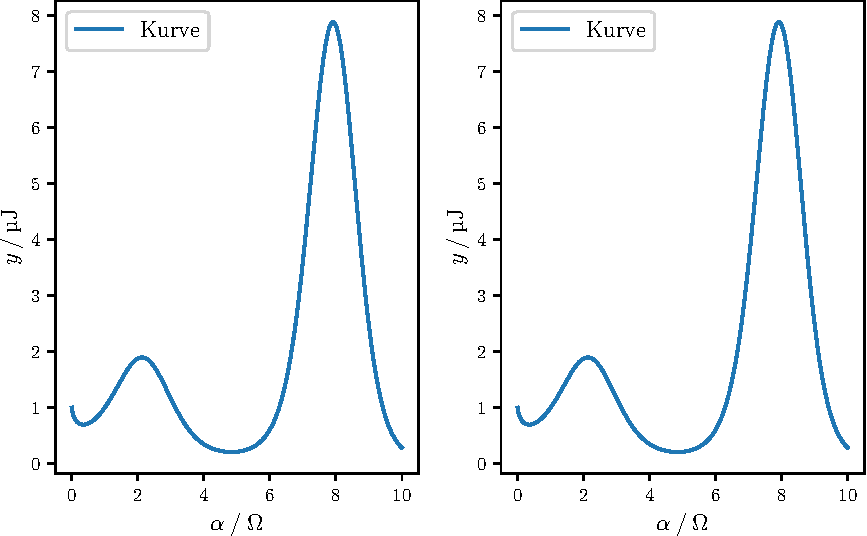
\includegraphics{plot.pdf}
  \caption{Temperaturverlauf der Messingstäbe außen.}
  \label{fig:T1T4}
\end{figure}
Die Verläufe haben alle eine kurzen Startbereich bis ca. $10 \,\si{\second}$ bei dem die Verläufe nicht
ansteigen. Danach stellt sich bei allen Verläufen eine Sättigungskurve ein.
Dabei fällt auf, dass der Temperaturverlauf des Edelstahlstabs am langsamsten
ansteigt und auch insgesamt die Form der Sättigungskurve abflacht.

\begin{figure}
  \centering
  \includegraphics{T5_T8.pdf}
  \caption{Temperaturverlauf von Aluminium und Edelstahl außen.}
  \label{fig:T5T8}
\end{figure}

\begin{figure}
  \centering
  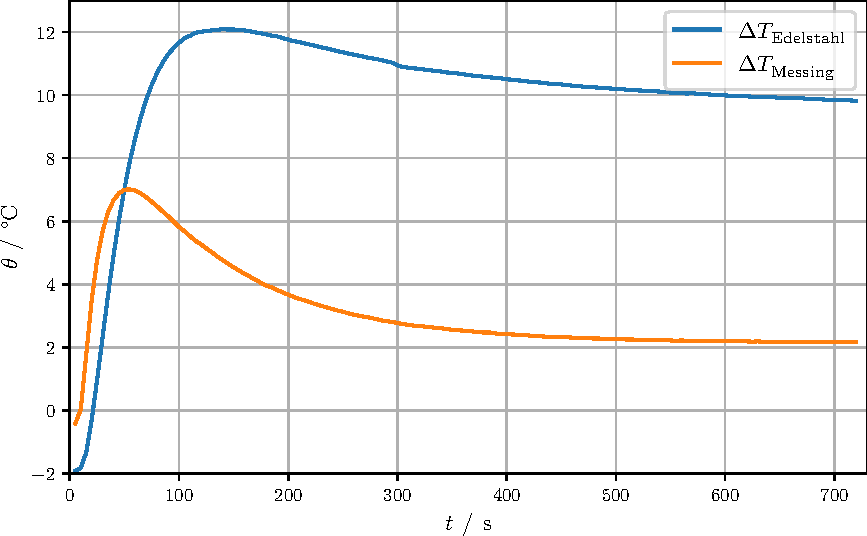
\includegraphics{Tempdiff.pdf}
  \caption{Temperaturdifferenz des breiten Messingstabs und des Edelstahlstabs.}
  \label{fig:Tempdiff}
\end{figure}

\subsection{Bestimmung des Stabs mit der höchsten Wärmeleitung}
\label{hoechste}

Nach ca. $700\,\si{\second}$ hat die höchste Temperatur erreicht.


\subsection{Dynamische Methode}
\label{dynam}

\begin{figure}
  \centering
  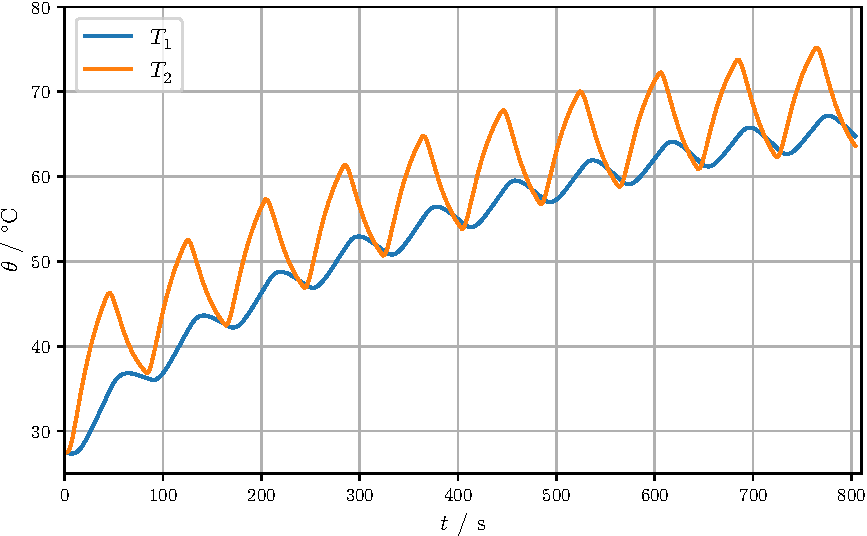
\includegraphics{80sMess.pdf}
  \caption{Temperaturverlauf des breiten Messingstabs.}
  \label{fig:80sMess}
\end{figure}

\begin{figure}
  \centering
  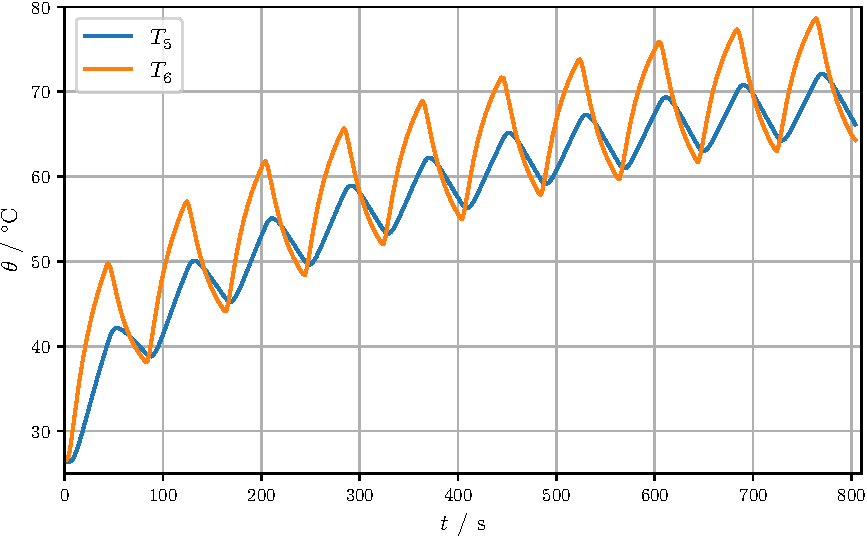
\includegraphics{80sAlu.pdf}
  \caption{Temperaturverlauf des Aluminiumstabs.}
  \label{fig:80sAlu}
\end{figure}

\begin{figure}
  \centering
  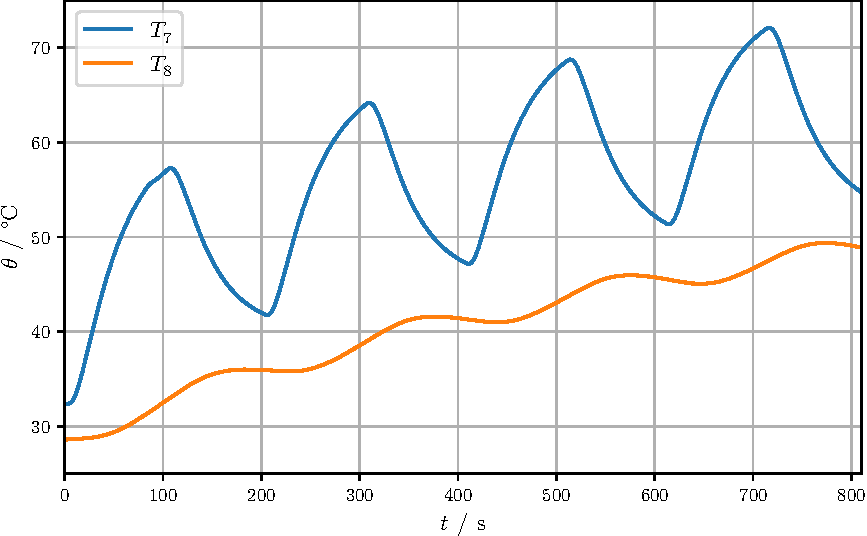
\includegraphics{200sEdelstahl.pdf}
  \caption{Temperaturverlauf des Edelstahlstabs.}
  \label{fig:200sEdelstahl}
\end{figure}
